This chapter contains an extensive explanation of the dataset and the labels and acoustic features that were extracted from it. I then introduce the architectures of the models I have created.


\section{The Data}
\label{sec:3.the_data}
As explained in the \nameref{sec:salami} section, I will be using the internet archives subset of the SALAMI dataset as data for the models I will create. Another benefit of using this dataset, apart from the amount of publicly available songs, is that the SALAMI dataset, and the internet archives subset in particular, have been part of the evaluation datasets for many MIREX Music Structural Segmentation contests. The results produced by the models I will create will therefore be quite comparable to the results reported in the many MIREX submissions to this specific MIREX contest.

The internet archives subset consists of two parts: A CSV file containing all metadata about each song and the actual annotations. Among this metadata is a web-link to the audio file of that song in mp3 format. Using these links and the SONG ID given to each song, each audio file was downloaded and saved as \textit{[song-id].mp3}.

All annotations for a song are stored in a folder named by the ID of the song. Since one or two annotators have annotated each song, this folder may contain one or two text files. Each line of text in these text files stand for a segment; the first number denote the time point (in seconds) of the start of the segment. Then the labels describing the function of the segment follow. Because two levels of annotation were used, the collection of labels may contain one or more items.

The first item in the collection of labels always is a lowercase letter describing the low level function of the segment, often written in combination with a \textit{'}. Segments with the same label are musically similar to each other, the \textit{'} means that although the (musical) function between the segments is similar, they differ slightly in musical terms (e.g. key, mode).

Some collections of labels contain two more labels, the high-level annotation (denoted by an uppercase letter) and the segment function (chorus, verse, etc.). All time points without high-level annotation and segment function implicitly have the most recent high-level annotation and segment function that occurred. 

Apart from the text files containing all annotations of one annotator, the folder with annotations also includes a folder for each annotator. In this folder there are multiple text files each one containing one type of annotation, thus one text file contains the low-level annotations, another one contains the segment functions, etc.

The exact instructions given to each annotator on how to annotate a song, and how to format their annotations can be found in the \href{https://github.com/DDMAL/salami-data-public/blob/master/SALAMI%20Annotator%20Guide.pdf}{annotator's guide (link)}.

Using the time points and labels of each segment boundary I will be able to evaluate the accuracy of each model to predict the start of each segment within a 0.5 second and 3 seconds tolerance, I will further explain the exact evaluation method in the \nameref{sec:eval_meth} section. The full list of songs used can be found in \autoref{app:dataset}.

\subsubsection{Label extraction}
\begin{table}[t]
    \centering
    \begin{tabular}{|l|l|l|l|}
    \hline
    \textbf{Label}         & \textbf{Occurrence in data} & \textbf{Grouped Label} & \textbf{Occurrence in data} \\ \hline\hline
    silence       & 446                & \textbf{silence}       & 446                \\ \hline
    no\_function  & 483                & \textbf{no\_function}  & 505                \\ \hline
    applause      & 12                 & no\_function  &                    \\ \hline
    stage\_sounds & 6                  & no\_function  &                    \\ \hline
    spoken        & 3                  & no\_function  &                    \\ \hline
    crowd\_sounds & 1                  & no\_function  &                    \\ \hline
    intro         & 243                & \textbf{intro}         & 300                \\ \hline
    head          & 57                 & intro         &                    \\ \hline
    verse         & 718                & \textbf{verse}         & 726                \\ \hline
    pre-verse     & 7                  & verse         &                    \\ \hline
    voice         & 1                  & verse         &                    \\ \hline
    interlude     & 189                & \textbf{interlude}     & 249                \\ \hline
    transition    & 51                 & interlude     &                    \\ \hline
    break         & 9                  & interlude     &                    \\ \hline
    solo          & 514                & \textbf{solo}          & 717                \\ \hline
    instrumental  & 160                & solo          &                    \\ \hline
    theme         & 39                 & solo          &                    \\ \hline
    main theme    & 4                  & solo          &                    \\ \hline
    chorus        & 655                & \textbf{chorus}        & 740                \\ \hline
    pre-chorus    & 61                 & chorus        &                    \\ \hline
    post-chorus   & 24                 & chorus        &                    \\ \hline
    bridge        & 106                & \textbf{bridge}        & 107                \\ \hline
    build         & 1                  & bridge        &                    \\ \hline
    outro         & 132                & \textbf{outro}         & 182                \\ \hline
    coda          & 48                 & outro         &                    \\ \hline
    fade-out      & 2                  & outro         &                    \\ \hline
    \end{tabular}
    \caption{Grouping of all 26 unique labels into 9 main labels.}
    \label{tab:label_grouping}
\end{table}
To not have to manually parse each text file I have made use of the formatted annotations in Json Annotated Music Specification (JAMS) format \cite{Humphrey2014jams}. These formatted annotations are available in the Music Structure Analysis Framework (MSAF) \cite{Nieto2016systematic}.

For each song in the internet archives dataset I've chosen the first annotation. This reduced the amount of different annotators to under 5, thereby decreasing the amount of ambiguity between the annotations of different songs. Still, there were quite a lot of different labels present in the dataset (26), of which 10 labels have around or under 10 occurrence within the 4000 segments present in the first annotation of each song in the internet archives dataset.

By decreasing the amount of unique labels, I further decreased the amount of ambiguity between the annotations and presumably increased the accuracy of the models. I've based the grouping on occurrence of the unique label in the dataset, its musical function and the label of another annotator for the same segment. By also listening to a few segments of each of the labels that had a low occurrence in the data, I could also use my own judgement of the relation between a certain label and its associated sounds for the grouping of the labels. 

One example are the segments that were labeled as \textit{instrumental}. These segments turned out to be musically equal to \textit{solo} in the context of the data. Since the data primarily consists of live recordings of (alternative) Western Popular Music, both meant a sole guitar (supported by drums) without any lyric. I therefore chose to group these labels together as \textit{solo}. For the other label groupings a similar process was performed as well, while the other factors described were taken into account as well. The final grouping of each label can be found in \autoref{tab:label_grouping}.

Once each raw label was converted to its grouped label, a one-hot-encoding vector of each label was created. A one-hot-encoding vector of a beat is a vector with the length of the amount of labels containing only zeros except for the index of the true label for that beat. The indices of the grouped labels are 0 to 8 for \textit{silence, no\_function, intro, verse, interlude, solo, chorus, bridge} and \textit{outro} in that specific order respectively.


\section{Feature Selection}
\subsubsection{Feature Extraction}
\begin{table}[t]
    \centering
    \begin{tabular}{|l|c|c|}
    \hline
    \textbf{Feature} & \textbf{Vector Length} & \textbf{Matrix Size}  \\ \hline\hline
    CQT       & 84          & $84\times4$  \\ \hline
    CENS      & 12          & $12\times4$  \\ \hline
    PCP       & 12          & $12\times4$  \\ \hline
    Tonnetz   & 6           & $6\times4$   \\ \hline
    MFCC      & 14          & $14\times4$  \\ \hline
    Tempogram & 192         & $192\times4$ \\ \hline
    \end{tabular}
    \caption{Vector length and matrix size of each feature extracted.}
    \label{tab:feature_sizes}
\end{table}
I used the LibROSA Python package for music and audio analysis \cite{Mcfee2015librosa} to extract the features from each audio file. I have used a hop length of 1024 together with a FFT window of 4096 for 75\% overlap within each feature vector.

First the beats were extracted using the method introduced by \textcite{Ellis2007beat}.
Then the Chroma Energy Normalized Statistics (CENS) \cite{Muller2005chroma} chroma variant was extracted. As low level harmonic/chroma features I extracted the Pitch Class Profile (PCP) \cite{Lee2006automatic}. I saved the PCP as self-contained feature and used it to create the Tonnetz features \cite{Harte2006detecting}. I also created a Mel Spectrogram \cite{Stevens1937scale} and used it to create the Mel-Frequency Cepstral Coefficients (MFCC) with 14 coefficients \cite{Logan2000mel}, these represent the timbre of the song. As other timbre feature I extracted the Constant-Q Transform (CQT) \cite{Brown1991calculation}, using the technique described by \textcite{Schorkhuber2010constant}. Because often a segment boundary goes hand in hand with a change in tempo (e.g. a short speedup in tempo, or the next segment is in a lower or higher tempo), I extracted the tempogram of each song with a window length of 192 \cite{Grosche2010cyclic}. 

The resulting feature vectors have a length of 84, 12, 12, 6, 14 and 192 for the CQT, CENS, PCP, Tonnetz, MFCC and tempogram feature vectors respectively (\autoref{tab:feature_sizes}).

\subsubsection{Data Reduction}
Each feature was first extracted based on the frames of a song. The amount of frames of a song is calculated by the sample rate (amount of audio samples per second) multiplied by the length of the song (in seconds) divided by the hop length. Each song is converted to Waveform (wav) audio format with a sample rate of 22050, this combined with a mean song length of 4 minutes or 240 seconds and a hop length of 1024 for each feature results in $(240\cdot22050)/1024=5168$ frames on average for each song. 

To reduce the amount of feature vectors I have beat synced each feature. The means that for each beat in a song there is one vector for each feature. This vector is calculated as the average of all vectors of that feature within the beat. With an average beats per minute (BPM) of 120 for all songs (thus 2 'frames' per second), the average amount of vectors per song is now reduced to $240\cdot2=480$. With a total of 377 songs (after data cleaning) I gathered a total of about 180000 vectors per feature.


\section{Proposed Architectures}
\subsection{Preserving Temporal Aspect of Music}
To obtain faster learning speeds of the models, the data needs to be shuffled; if all beats of a song are kept in the initial order, the output labels will be sequences of the same label. Even when the batch size is increased, samples with the same output label are still being fed to the network in each learning iteration, thus lowering its capabilities to learn multiple output labels in one learning iteration.

One problem of shuffling the data however is that one beat alone will not be enough for a network to learn all patterns that can be associated with an output label, thus requiring the temporal aspect of the song to be intact. My proposed solution to this problem is to, instead of using a single vector per feature per beat, combine the vectors of two beats before the current beat, the vector of the current beat and the vector of the beat after the current beat into a matrix for each feature. The results is therefore a matrix, with a shape of $length\_feature\times4$, per feature per beat.

In the next sections I will explain, per proposed model, how I use this matrix as input.

\subsection[CNN]{Convolutional Artificial Neural Network}
\begin{figure}[t]
    \centering
    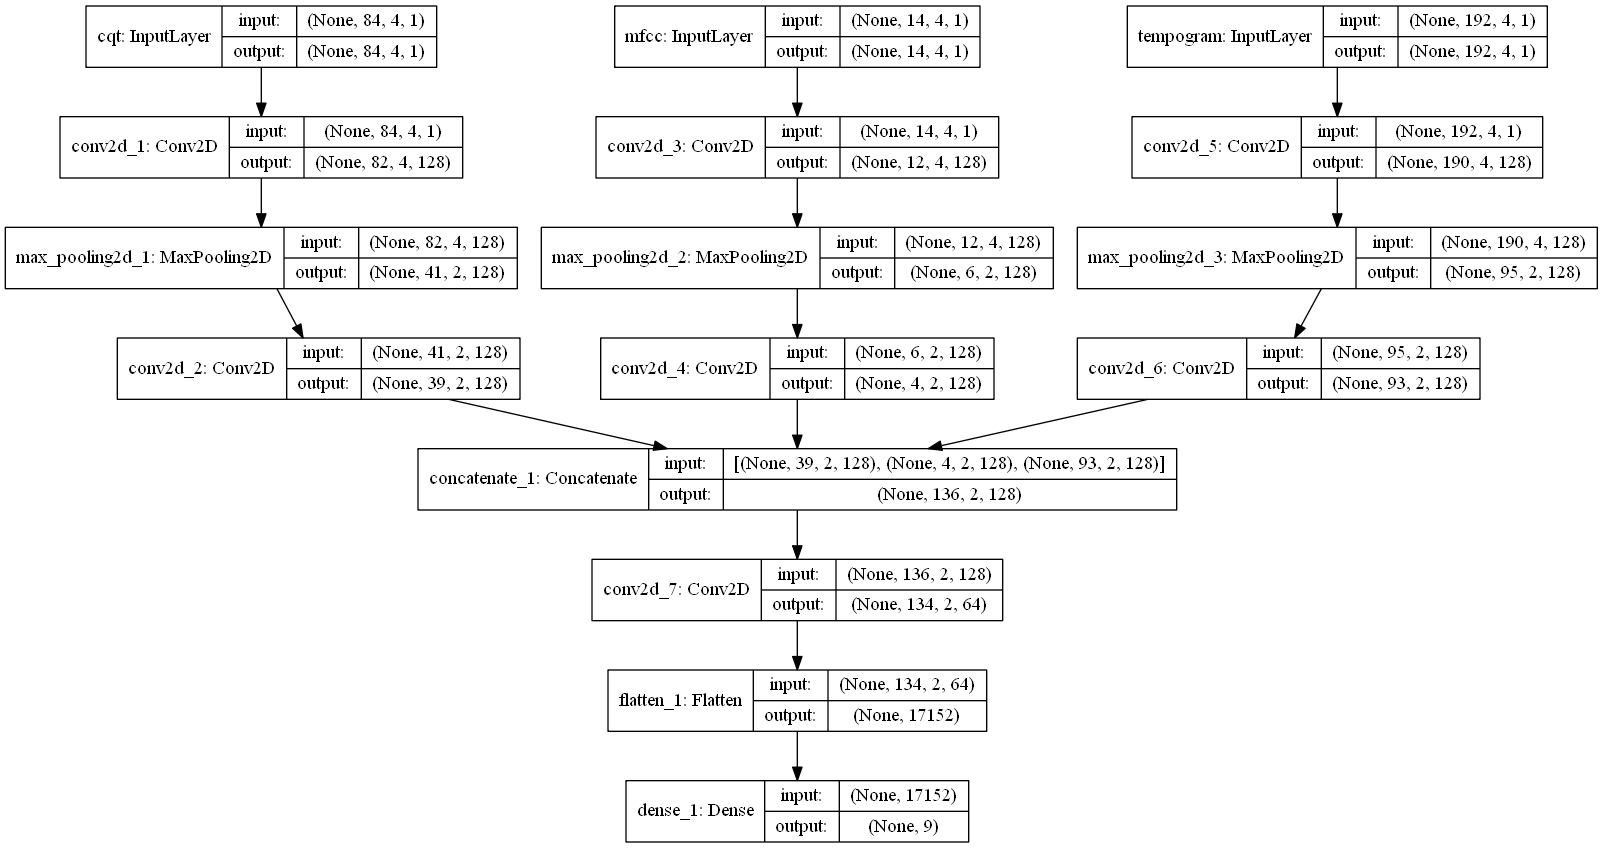
\includegraphics[width=1\textwidth]{images/cnn_architecture}
    \caption{Proposed CNN architecture with CQT, MFCC and Tempogram as example inputs.}
    \label{fig:proposed_cnn_architecture}
\end{figure}
Because of the great results with convolutional neural networks in the music structure analysis field, I propose an implementation of the segmentation approach using a convolutional neural network. 

This CNN has multiple input layers, one matrix per beat for each feature used. Each input matrix will therefore act as the input image, as described in the \nameref{sec:cnn_related} section. After each input layer there is a two-dimensional convolutional layer with a $3\times1$ kernel, followed by a possible two-dimensional max- or average-pooling layer with a $2\times2$ pooling size. Then another two-dimensional convolutional layer follows with 128 neurons and $3\times1$ kernel.

The outputs of this last convolutional layer of each input is then concatenated to one big $n\times4$ matrix. $n$ represents the summed length of the first dimension of each output shape. The concatenated outputs are then fed into a last two-dimensional convolutional layer, with 64 neurons and $3\times1$ kernel.

The (two-dimensional) output of the final convolutional layer is flattened into a single vector, and used as input for a dense layer with 9 neurons (each neuron representing one output label) and \textit{softmax} activation function. The softmax activation function normalizes the outputs of each neuron into a probability distribution, thus each output is scaled to be within the [0,1] interval and all scaled outputs sum to 1. The highest output is then selected as predicted label for the input, with its activation as confidence or probability that this label is the true label.

An example model, with CQT, MFCC and Tempogram as input features can be found in \autoref{fig:proposed_cnn_architecture}.

\subsection[Bi-LSTM]{Bi-Directional Long Short-Term Memory Artificial Neural Network}
\begin{figure}[t]
    \centering
    \begin{subfigure}{\textwidth}
        \centering
        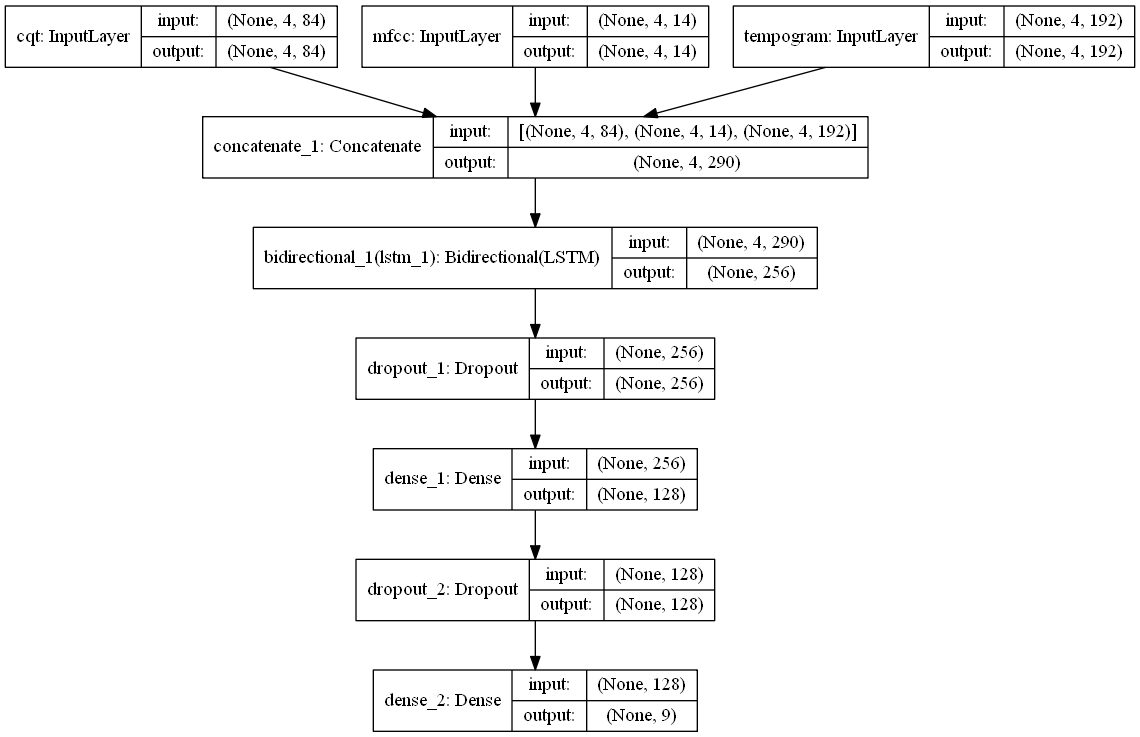
\includegraphics[width=.9\linewidth]{images/lstm_architecture_single}
        \caption{Single LSTM layer architecture.}
        \label{fig:lstm_single}
    \end{subfigure}
    \par\bigskip
    \begin{subfigure}{\textwidth}
        \centering
        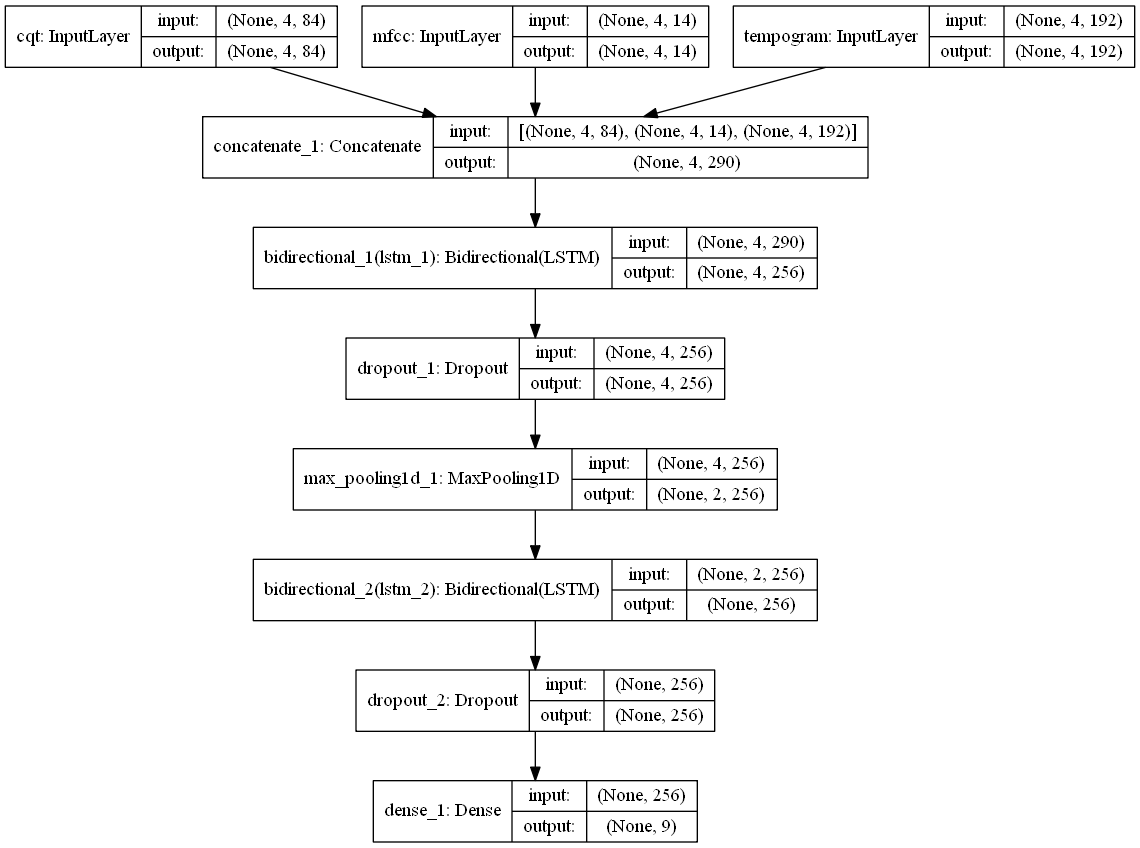
\includegraphics[width=.9\linewidth]{images/lstm_architecture_multi}
        \caption{Double LSTM layer architecture.}
        \label{fig:lstm_double}
    \end{subfigure}
    
    \caption{Proposed LSTM architectures with CQT, MFCC and Tempogram as example inputs.}
    \label{fig:proposed_lstm_architecture}
\end{figure}
Alongside a convolutional neural network, I also propose a bi-directional long short-term memory neural network implementation of the segmentation by annotation approach. This model will show if its capabilities to cope with temporal data and its performance in the automatic audio segmentation field also apply to music structure detection. The model is made bi-directional because of the reported increased performance of bi-directional recurrent neural networks over normal recurrent neural networks \cite{Schuster1997bidirectional}.

I propose two different architectures using long short-term memory units, a model with one bi-directional LSTM layer (\autoref{fig:lstm_single}), and a model with a double bi-directional LSTM layer, optionally combined with a max- or average-pooling layer (\autoref{fig:lstm_double}). Both models first contain an input layer per feature used, similar to the proposed CNN. In contrast to the CNN, all input is immediately concatenated into one matrix (with shape $n\times4$).

When a single LSTM layer model is build, this matrix is fed into bi-directional LSTM layer. However, since an (B-)LSTM layer has only one dimension, each column (or vector representing a beat) is separately evaluated. Because we want a single output from the full network, the B-LSTM layer is set to put one vector out after all 4 beats have been evaluated. This output is then passed into a dense layer, containing 128 neurons, whose output ultimately is put in a dense layer containing 9 neurons (each one representing one output label), and a \textit{softmax} activation function (\autoref{fig:lstm_single}).

If a double LSTM layer model is built the first B-LSTM layer does not first evaluate all 4 beats, but gives an output for each of the 4 beats. Each output is optionally passed through a one dimensional max- or average-pooling layer with a pool size of 2. Then another B-LSTM layer receives each output and evaluates all four, before outputting a single vector which is fed into the final dense layer with 9 neurons and softmax activation (\autoref{fig:lstm_double}).